\chapter{Saliency Maps}
\label{cha:saliency}
Das Saliency Map Verfahren wurde erstmals von den Neurowissenschaftlern Itti et al. \cite{itti_model_1998} in ihrer Studie vorgeschlagen. Die Studie beschreibt eine Methode zur Extraktion von einzigartigen Merkmalen, wie beispielsweise Farben, Farbintensitäten und Strukturen, sogenannten High-Level Features, aus Bildern, die wiederum in sogenannten Saliency Maps topografisch visualisiert werden. Diese High-Level Features sind nichts anderes als spezifische Pixel im Bild auf Mikroebene (Low-Level Features), welche die optisch ansprechendsten respektive bedeutendsten Stellen in einem Bild repräsentieren. 

Um also spezifischen Bildmerkmalen eine semantische Bedeutung zuzuordnen, werden beispielsweise Farbbilder anhand des Saliency Map Verfahrens in Schwarzweißbilder umgewandelt, um die stärksten darin vorhandenen Farben zu analysieren und zu extrahieren.

\section{Konzept}
\label{cha:saliency_konz}
Bei \ac{CNN} werden Merkmale von Eingabebildern extrahiert, indem zunächst im Input-Layer Low-Level Features und mit jeder weiteren Schicht des Netzwerks immer komplexere Merkmale (High-Level Features), wie etwa Kanten, Rundungen oder Strukturen erlernt werden \cite{stanford_unsupervised_tutorial}.

Diese Kenntnis um \ac{CNN} und Saliency Maps machten sich Simonyan et. al erstmalig im Kontext von Deep Learning zunutze, um die gelernten Merkmale des zugrunde liegenden \ac{CNN} anhand von Saliency Maps zu visualisieren \cite{simonyan_deep_2013}. 
Die in der Arbeit von Simonyan et. al erzeugten Bilder sind hierbei nicht oder nur ansatzweise für den Menschen erkennbar, wurden jedoch vom zugrunde liegenden \ac{CNN} mit einer hohen Konfidenz richtig klassifiziert werden.
~\newline

Aus dieser Kenntnis ergeben sich folgende Hypothesen:
\begin{itemize}
	\item Ein Convolutional Neural Network mit beliebiger Architektur, jedoch trainiert mit demselben Datensatz (\ac{GTSRB}) wie das Black Box Modell (aus der Aufgabenstellung), lässt sich ähnlich gut angreifen wie das Black Box Modell selbst.
	\item 	Saliency Maps repräsentieren die wesentlichen Merkmale, die das Convolutional Neural Network zu den Eingabebildern gelernt hat. Die erzeugten Bilder mit dem Saliency Map Verfahren werden wiederum vom \ac{CNN} mit einer hohen Konfidenz richtig klassifiziert, das heißt das jeweils erzeugte Bild wird vom \ac{CNN} als Verkehrszeichen erkannt und mit hoher Konfidenz richtig klassifiziert, ist jedoch für den Menschen nicht als solches erkennbar.
\end{itemize}

%Ein verbreitetes Verfahren aus dem Bereich Computer Vision zur Visualisierung relevanter Pixel ist die Erstellung von \textit{Saliency Maps} (dt. Ausprägungskarten). Diese können verwendet werden, um die Qualität, sprich Aussagekraft, jedes einzelnen Bildpunkts ersichtlich zu machen. Simonyan et al. \cite{simonyan_deep_2013} führt die grundlegende Methodik entsprechend Saliency Maps weiter aus und unterscheidet zwischen einer allgemeinen “'Klassen-Definierenden”' Saliency Map sowie einer Saliency Map zu einem gegebenen Eingabebild entsprechend der Zielklassen.
%
%
%Gebräuchliche Anwendung dieses Verfahrens im Machine Learning Bereiches betreffen der Darstellung von High Level Features einzelner Neuronen \cite{liu_delving_2016} im Bezug auf eine gezielte Klasse. Diesen Ansatz weiterverfolgend, entsprechen die erzeugten Saliency Maps im letzten Layer einer starken Neuronenaktivierung, die einer "'High Level”' Darstellung der gezielten Klasse entspricht, die vom \ac{NN} für das Bild errechnet wurde. 
%
%
%Diese Saliency Map sollte also im Rückschluss mit einer hohen Konfidenz bezüglich der entsprechenden Klasse klassifiziert werden, wenn das erzeugte Bild als Eingabe verwendet wird. Daraus ergibt sich die Hypothese, mit Hilfe dieser Visualisierung für den Menschen semantisch nicht erkennbare Verkehrszeichen Bilder zu erzeugen, die hohe Zielkonfidenzen von 0.9 oder mehr erreichen. Die beschriebene Methode wird in der Implementierung als “'Vanilla Saliency”' bezeichnet.


\section{Implementierung}

Als vorverarbeitenden Schritt werden zunächst alle 12.630 Bilder aus dem GTSRB-Testdatensatz, welche in 24-Bit Farbtiefe und im \ac{PPM} Dateiformat vorliegen, in das \ac{PNG} Dateiformat konvertiert und im Dateisystem abgespeichert.


Ein eigenes \ac{CNN} Modell („Aphrodite“) wird mit dem \ac{GTSRB}-Datensatz trainiert.

Die  vorliegenden \ac{PNG}-Bilder werden anhand dem „Aphrodite“-Modell klassifiziert:
Nur diejenigen Bilder, welche vom „Aphrodite“-Modell mit einer Konfidenz von 100\% korrekt klassifiziert wurden (3.063/12.630) werden im Dateisystem in einem eigenständigen Verzeichnis abgespeichert.

~\newline
Gemäß einer auf die Anforderungen an die Aufgabenstellung abgewandelten Variante zu Anh \cite{anh_implementations_2019}, erfolgt nun die Implementierung der verschiedenen Saliency Map Verfahren.

~\newline
Hierzu werden zunächst die drei Basismethoden „Vanilla“ \cite{simonyan_deep_2013}, „Guided Backpropagation“ \cite{springenberg_striving_2014} und „Integrated Gradient“ \cite{sundararajan_axiomatic_2017} implementiert. 
Unter Hinzufügung von Zufallsrauschen, gemäß \cite{smilkov_smoothgrad:_2017}, werden die Basismethoden verbessert, wie die Gegenüberstellung der Ergebnisse zu den eingesetzten Verfahren in Kapitel \ref{sec:SalErgebnisse} verdeutlicht.
Diese optimierten Varianten werden als „Smoothed Vanilla“, „Smoothed Guided Backpropagation“ und „Smoothed Integrated Gradient“ bezeichnet und implementiert.

~\newline
Jedes der Saliency Map Verfahren wird auf die in Schritt 3 erzeugten Bilder angewendet. Diese Bilder werden nacheinander vom Dateisystem geladen und anschließend auf eine Zielbildgröße von $64 \times 64 $ Pixel skaliert. 
Zur Extraktion und Visualisierung der gelernten Merkmale des zugrunde liegenden Modells (Aphrodite) zu jedem skalierten Eingabebild, wird das gewählte Saliency Map Verfahren auf jedes Eingabebild, unter Verwendung des trainierten „Aphrodite“-Modells, angewendet. 
Die damit erzeugten Bilder werden anschließend in einem nach dem verwendeten Saliency Map Verfahren bezeichneten Verzeichnis in der Größe $64 \times 64 $ Pixel im Dateisystem abgespeichert.

~\newline
Zur abschließenden Evaluierung der erzeugten Bilder am Black Box Modell, werden alle Bilder zu jedem eingesetzten Saliency Map Verfahren im Zyklus von 60 Bilder pro Minute (Übertragungslimit pro Minute an der Remote-Webschnittstelle) an das Trasi-Webinterface gesendet. Die Informationen, das heißt die vom Black Box Modell erkannte Zielklasse und Konfidenz, werden anschließend aus dem HTTP-Responsecode zu jedem übermittelten Bild in zwei verschiedenen Logdateien gespeichert: Die erste Logdatei speichert alle Ergebnisse aus dem jeweiligen HTTP-Responsecode, wohingegen die zweite Logdatei nur gefilterte Ergebnisse, das heißt Konfidenzen von mehr als 90\%, zu den übermittelten Bildern enthält.


%
%Nachfolgend wird der vollständige Datensatz lokal am eigenen Modell klassifiziert und alle Bilder mit einer Konfidenz von 100\% separat gesammelt. 
%
%Die vorgestellten Verfahren Vanilla Saliency\cite{simonyan_deep_2013}, Guided Backpropagation\cite{springenberg_striving_2014} und Integrated Gradient\cite{sundararajan_axiomatic_2017} werden jeweils in einer ungefilterten und und geglätteten Variante verwendet entsprechend einer auf die Aufgabenstellung angepasster Implementation auf der Basis von \cite{anh_implementations_2019}. 
%
%Ausgegeben wird ein Graustufenbild in der die relevanten Pixelbereiche durch hellere Einfärbung gekennzeichnet werden.
%
%Diese Bilder wurden danach an das Trasi Webinterface geschickt und das Resultat der Klassifikation abgespeichert. Zusätzlich wird pro Verfahren ein Logfile erstellt, welches alle Bilder mit einer Konfidenz >0.9 sowie die geschätzte Klasse und das Ursprungsbild festhält.
%

\section{Ergebnisse}
\label{sec:SalErgebnisse}
Mit den verschiedenen Saliency Map Verfahren wurden Graustufenbilder erzeugt, in denen die relevanten Bildmerkmale durch helle Pixeleinfärbungen gekennzeichnet sind. 
Die erzeugten Bilder sind hierbei vom Menschen nicht als Verkehrszeichen wahrnehmbar.

Die mit den Basismethoden „Vanilla“, „Guided Backpropagation“ und „Integrated Gradient“ erzeugt Bilder wurden vom Black Box Modell mit jeweils 45,834911\% als „Baustelle“ klassifiziert.
Dieses Ergebnis lässt sich möglicherweise auf die besonderen „Faltungseigenschaften“ von Convolutional Neural Networks zurückführen, dass wesentliche bildcharakterisierende Merkmale und die damit verbundene semantische Information aus den erzeugten Bildern verloren ging.

Dahingegen konnten mit den optimierten Saliency Map Verfahren („Smoothed Vanilla“, „Smoothed Guided Backpropagation“ und „Smoothed Integrated Gradient“) Bilder erzeugt werden, die Zielkonfidenzen von mehr als 90\% am Black Box Modell erreichten.

%Aus der Implementation konnten folgende Ergebnisse zu den 6 vorgestellten Variationen gesammelt werden. 
%
%Alle ungeglätteten Verfahren konnten keine positiven Ergebnisse bezüglich der Bilderzeugung mit einer Konfidenz $> 0.9$ liefern. Dies lässt sich möglicherweise auf die besonderen Einschaften von \acp{CNN} zurückführen, dass ohne Glättung in dem - ohne farbkanäle - bereits dimensionsreduziertem Bild keine ausgeprägten Kanten vorhanden sind und nach dem "'Falten"' Informationen verloren gehen. Desweiteren konnte am Blackbox Modell beobachtet werden, dass alle erzeugten ungegeglätteten Saliency Maps mit einer Konfidenz von $0.45834911$ als Klasse "'Baustelle"' erkannt werden.
%
%Dahingegen konnten bei allen geglätteten Varianten Bilder erzeugt werden, die vom Blackboxmodell mit hoher Sicherheit eine Klasse zugeordnet wurden. Es konnten einige unerwarteten Anomalien bei der Klassifizierung am Fremdmodell beobachtet werden.  Tabelle \ref{tab:sal1} zeigt wie aus Bild 5.1a (Höchstgeschwindigkeit (30))  mit den Verfahren "'Smoothed Guided Backpropagation"' (vgl. 5.1b) und "'Smoothed Vanilla Saliency"' (vgl. 5.1c) ein Bild erzeugt, welche mit einer Konfidenz >0.9 vom Webinterface erkannt wurden. Dabei muss beachtet werden, dass die Bilder als unterschiedliche Klassen eingestuft wurden. "'Vanilla Saliency"' stimmt überein (Höchstgeschwindigkeit (30), Konfidenz 0.9283), "'Guided Backpropagation"' wurde vom Fremdmodell einer anderen Klasse zugeordnet (Überholverbot, Konfidenz 0.9155).


\begin{table}
	\centering
	\begin{tabular}{p{4.5cm}p{4.5cm}p{4.5cm}}
		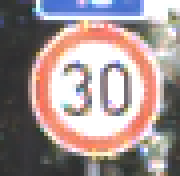
\includegraphics[width=\linewidth]{Images/AnPe/10771} & 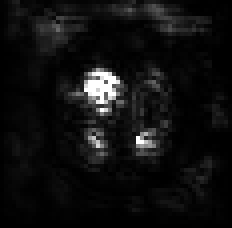
\includegraphics[width=\linewidth]{Images/AnPe/10771_guided} &
		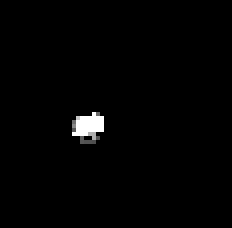
\includegraphics[width=\linewidth]{Images/AnPe/10771_vanil}\\ 
		5.1a: Ursprungsbild &5.1b: Guided Backprop. &5.1c: Vanilla Saliency \\
		Höchstgeschwindigkeit (30) & Überholverbot & Höchstgeschwindigkeit (30)\\
		& 0.9155 & 0.9283\\
		
	\end{tabular} 

	\caption{Ergebnisse von verschiedenen Verfahren am selben Bild. }
	\label{tab:sal1}
\end{table}

~\newline
Tabelle \ref{tab:sal1} zeigt exemplarisch, wie aus dem Ursprungsbild (5.1a „Höchstgeschwindigkeit (30)“), unter Verwendung des „Smoothed Guided Backpropagation“ Verfahrens, ein Bild erzeugt wurde, das vom Black Box Modell mit 91,55\% als „Überholverbot“ klassifiziert wurde (5.1b). 
Das „Smoothed Vanilla Saliency“ Verfahren erzeugte hingegen aus demselben Ursprungsbild ein Bild, das mit einer Zielkonfidenz von 92,83\% vom Black Box Modell als „Höchstgeschwindigkeit (30)“ erkannt wurde (5.1c).
%\begin{figure}
%	\begin{subfigure}{.33\textwidth}
%		\centering
%		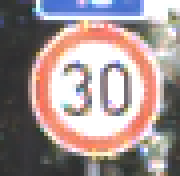
\includegraphics[width=.8\linewidth]{Images/AnPe/10771}
%		\caption{Ursprungsbild (Höchstgeschwindigkeit 30)}
%		\label{fig:ursprung1}
%	\end{subfigure}%penis
%	\begin{subfigure}{.33\textwidth}
%		\centering
%		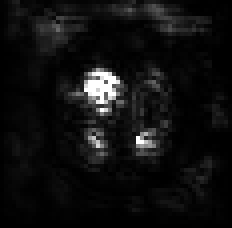
\includegraphics[width=.8\linewidth]{Images/AnPe/10771_guided}
%		\caption{Halblabor.}
%		\label{fig:salmap1}
%	\end{subfigure}
%	\begin{subfigure}{.33\textwidth}
%		\centering
%		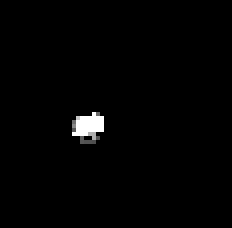
\includegraphics[width=.8\linewidth]{Images/AnPe/10771_vanil}
%		\caption{Freie Umgebung.}
%		\label{fig:salmap_1}
%	\end{subfigure}
%\end{figure}


~\newline
Tabelle \ref{tab:sal2} veranschaulicht weitere Beispiele für erfolgreich erzeugte Bilder, unter Verwendung der optimierten Saliency Map Verfahren. Wieder kann beobachtet werden, dass die erzeugten Bilder zwar mit einer Zielkonfidenz von mehr als 90\% vom Black Box Modell klassifiziert wurden, die ursprüngliche Klasse jedoch abweicht.

\begin{table}
	\centering
	\begin{tabular}{p{4.5cm}p{4.5cm}}
		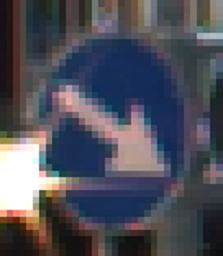
\includegraphics[height=4.4cm]{Images/AnPe/11240} &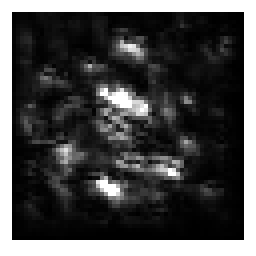
\includegraphics[width=\linewidth]{Images/AnPe/11240_guided}  \\
		& Guided Backprop.\\
		Rechts Vorbei & Einmalige Vorfahrt\\
		& 0.9678\\
		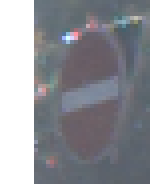
\includegraphics[height=4.4cm]{Images/AnPe/06848} &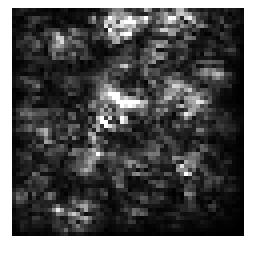
\includegraphics[width=\linewidth]{Images/AnPe/06848_s_int}  \\
		& Integrated Grad.\\
		Einfahrt Verboten & Überholverbot\\
		& 0.9571\\
		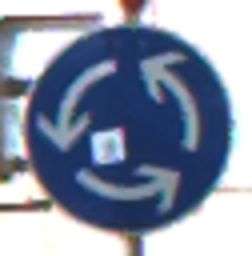
\includegraphics[height=4.4cm]{Images/AnPe/04709} &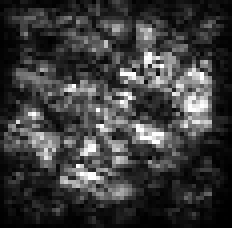
\includegraphics[width=\linewidth]{Images/AnPe/04709_int_grad}  \\
		& Integrated Grad.\\
		Kreisverkehr &Baustelle \\
		& 0.9999
	\end{tabular}
	\caption{Weitere Beispiele für Irrbilder mit Konfidenz >0.9 inklusive entsprechendem Ursprungsbild und verwendetem Verfahren.}
\label{tab:sal2}
\end{table}

%\begin{table}
%	\centering
%	\begin{tabular}{p{4.4cm}p{4.4cm}p{4.4cm}}
%		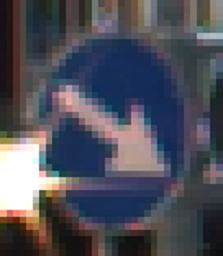
\includegraphics[height=4.4cm]{Images/AnPe/11240}&
%		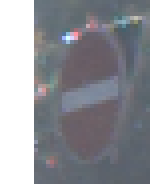
\includegraphics[height=4.4cm]{Images/AnPe/06848}&
%		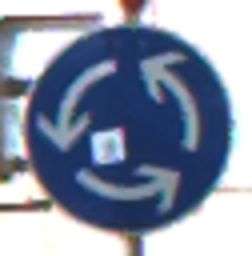
\includegraphics[height=4.4cm]{Images/AnPe/04709}\\
%		Rechts Vorbei & Einfahrt Verboten & Kreisverkehr\\
%		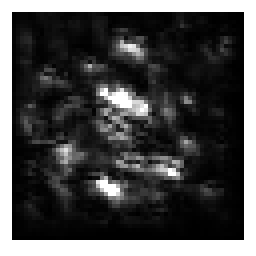
\includegraphics[width=\linewidth]{Images/AnPe/11240_guided} &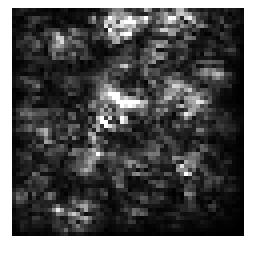
\includegraphics[width=\linewidth]{Images/AnPe/06848_s_int}  &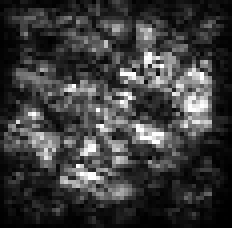
\includegraphics[width=\linewidth]{Images/AnPe/04709_int_grad}  \\
%		Guided Backprop.& Integrated Grad.& Integrated Grad.\\
%		Einmalige Vorfahrt& Überholverbot&Baustelle\\
%		0.9678& 0.9571& 0.9999\\
%	\end{tabular}
%	\caption{Weitere Beispiele für Irrbilder mit Konfidenz >0.9 inklusive entsprechendem Ursprungsbild und verwendetem Verfahren.}
%	\label{tab:sal2}
%\end{table}


Zusammenfassend konnte hiermit gezeigt werden, dass die in Kapitel \ref{cha:saliency_konz} formulierten Hypothesen zutreffen und sich Bilder – unter Verwendung eines eigens trainierten \ac{CNN} Modells („Aphrodite“) sowie verschiedener Saliency Map Verfahren – erzeugen lassen, die zwar keine für den Menschen sinnvolle Bedeutung haben, jedoch beim Black Box Modell Zielkonfidenzen von mehr als 90\% erreichten.


%Zusammenfassend konnte gezeigt werden, dass es mithilfe der Erstellung von Saliency Maps an einem eigenen Modell Bilder erzeugt werden können, welche von einem unbekanntem \ac{NN} mit hohen Konfidenzen verschiedenen Klassen zugeordnet werden. Die Erfolgsrate in Relation zur Anzahl erzeugter Bilder und dem Rechenaufwand ist dabei jedoch gering und es herrscht aktuell keine verlässliche Aussagekraft darüber, welcher Klasse das erzeugte Bild zugeordnet wird. 
